\documentclass[a4paper,12pt]{article}
\usepackage[utf8x]{inputenc}
\usepackage{ucs}
\usepackage[german]{babel}
\usepackage{fontenc}
\usepackage{graphicx}
\usepackage{tabularx}		% gescheite Tabellen
\usepackage{multirow}
\usepackage{fullpage}		% weniger rand
\usepackage{hyperref}
\usepackage{url}
\usepackage[numbers]{natbib}	% literaturliste
\usepackage{listings}		% codelistings
\usepackage{color}
\usepackage{xspace}
\usepackage{longtable, lscape}
\usepackage[onehalfspacing]{setspace} % Zeilenabstand

\newcommand\EBP{\textit{Elektronische Betreuungsplanung}\xspace}

\newcolumntype{R}{>{\raggedright\arraybackslash}X}	% spaltenstil für tabelle

\citeindextrue

\lstset{
	language=bash,
	basicstyle=\footnotesize,	% the size of the fonts that are used for the code
	numbers=left,			% where to put the line-numbers
	numberstyle=\footnotesize,	% the size of the fonts that are used for the line-numbers
	stepnumber=1,			% the step between two line-numbers. If it's 1, each line will be numbered
	numbersep=5pt,			% how far the line-numbers are from the code
	backgroundcolor=\color{white},	% choose the background color. You must add \usepackage{color}
	showspaces=false,		% show spaces adding particular underscores
	showstringspaces=false,		% underline spaces within strings
	showtabs=false,			% show tabs within strings adding particular underscores
	frame=single,			% adds a frame around the code
	tabsize=4,			% sets default tabsize to 2 spaces
	captionpos=b,			% sets the caption-position to bottom
	breaklines=true,		% sets automatic line breaking
	breakatwhitespace=false,	% sets if automatic breaks should only happen at whitespace
	title=\lstname,			% show the filename of files included with \lstinputlisting; also try caption instead of title
	escapeinside={\%*}{*)},		% if you want to add a comment within your code
	morekeywords={*,...}		% if you want to add more keywords to the set
}

% damit tex nicht wegen umlauten etc abschmiert beim listingparsen
\lstset{literate=
	{Ö}{{\"O}}1
	{Ä}{{\"A}}1
	{Ü}{{\"U}}1
	{ß}{{\ss}}2
	{ü}{{\"u}}1
	{ä}{{\"a}}1
	{ö}{{\"o}}1
	{°}{{\textdegree}}1
}


%opening
\title{Dokumentation\\Elektronische Betreuungsplanung\\(EBP)}
\author{Sebastian Kumminger \\
	Tobias Himmer \\
	Fabian Schneider}

\begin{document}

\maketitle

\newpage

\tableofcontents

\listoffigures

\listoftables

\newpage

\section{Projektablauf}

\subsection{Anforderungsdefinitionen}

\subsubsection{Ausgangssituation und Zielsetzung}
\label{subsubsec:ziel}
Das Ziel ist es, eine Applikation zu entwickeln, die es Einrichtungen der Behinderten- und Altenhilfe ermöglicht,
die langfristige Betreuungsplanung mit der Tagesdokumentation zu verknüpfen. Es sollen Ereignisse aus dem Tagesgeschehen,
die in der Tagesdokumentation der Wohngruppe / des Pflegeheims erfasst werden,
der Betreuungsplanung des betroffenen Bewohners zugeordnet werden können.
Damit soll doppelter Dokumentationsaufwand verhindert werden.
Die Software soll in stationären und ambulanten Einrichtungen der Behindertenhilfe in Baden Württemberg eingesetzt werden. 
Diese Einschränkung ergibt sich aus der Implementierung der Betreuungsplanung. Diese Version orientiert sich an dem aktuell in Baden Württemberg
geltenden 
Standard, dem Metzler-Verfahren. 
Die Software soll vorwiegend von pädagogischen Fachkräften benutzt werden. Entsprechend den individuellen Arbeitsabläufen in den 
Einrichtungen der Behindertenhilfe ist auch eine Bedienung durch Personal auf Leitungsebene (Heimleitung) denkbar\cite{Pflichtenheft}.

Die fachlichen Anforderungen an die \EBP wurden gemeinsam mit Herrn Martin Zimmer (Koordinator Unternehmensbereich II des DRK-Sozialwerks in
Bernkastel-Wittlich) erarbeitet und ausformuliert. Ergebnis dieser Arbeit sind die folgenden User Stories.

\subsubsection{User Stories}
\label{subsubsec:userstories}
User Stories sind ein Ansatz aus der Agilen Softwareentwicklung, um die Anforderungen verschiedener User an die Software zu definieren. Die
Formulierung einer User Story erfolgt nach folgendem Template \cite{Wikipedia_User_Story}:
\begin{lstlisting}
As a <role>, I want <goal/desire> so that <benefit>
\end{lstlisting}
Oder in der verkürzten Form:
\begin{lstlisting}
As a <role>, I want <goal/desire>
\end{lstlisting}
User Stories, die thematisch im Zusammenhang stehen werden unter einem Epic zusammengefasst. Die Sprache sollte bei der Formulierung
 von Epic und User Stories aus der Lebenswelt des Kunden stammen. Die Anforderungen an die \EBP wurden in folgende Epic und User Stories aufgeteilt:
\newline

\begin{longtable}{| p{0.25\textwidth}|p{0.05\textwidth}|p{0.7\textwidth} | }
  \hline
 \textbf{Epic} & \textbf{Nr.} & \textbf{User Story} \\
  \hline
\multirow{4}{0.25\textwidth}{Die persönlichen Daten eines Klienten sollen digital verwaltet werden} & 1 & Als Pflegekraft kann ich die Kontaktdaten eines Klienten anzeigen lassen und auch bearbeiten.  \\
  \cline{2 -3}
& 2 & Als Pflegekraft kann ich Informationen über die Leistungsträger der Klienten in meinem Verantwortungsbereich anzeigen lassen und
auch bearbeiten.\\
   \cline{2 - 3}
& 3 & Als Pflegekraft kann ich für die Klienten in meinem Verantwortungsbereich anzeigen lassen, welche freiheitseinschränkenden
Maßnahmen richterlich angeordnet werden, um Rechtssicherheit bei meiner Arbeit zu erlangen.\\
   \cline{2 - 3}
& 4 & Als Pflegekraft kann ich die gesetzliche Betreuung und die institutionelle Bezugsbetreuung anzeigen lassen und auch bearbeiten.\\
  \hline
\multirow{3}{0.25\textwidth}{Für jeden Klienten können mehrere Projekte organisiert werden, die eine pädagogische Zielsetzung haben} & 5 & Als für ein Projekte verantwortlicher Mitarbeiter kann ich neue Projekte anlegen \\
 \cline{2 - 3}
  & 6 & Als für ein Projekte verantwortlicher Mitarbeiter kann ich pädagogische Ziele für ein Projekt definieren \\
   \cline{2 - 3}
  & 7 & Als Pflegekraft kann ich Textfragmente aus der Zielsetzung oder der Projektbeschreibung in einen bestimmten
Bereich der Betreuungsdokumentation übertragen, um den Fortschritt und die Zielerreichung der Langzeitplanung einfach dokumentieren zu können.\\
 \hline
\multirow{4}{0.25\textwidth}{Bei Besprechungen mit einem Klienten müssen Protokolle erstellt werden. Diese Protokolle sollen Teil der \EBP sein.} & 8 & Es können für jeden Klienten mehrere Protokolle angelegt werden. \\
\cline{2 - 3}
 & 9  & Bei jedem Protokoll sind die Teilnehmer und das Protokolldatum ersichtlich. \\
\cline{2 - 3}
& 10 & Ein oder mehrere Teilnehmer können als Protokollant markiert werden \\
\cline{2 - 3}
& 11 & Als Pflegekraft kann ich Textfragmente aus dem Protokolltext in einen bestimmten
Bereich der Betreuungsdokumentation übertragen, um den Fortschritt und die Zielerreichung der Langzeitplanung einfach dokumentieren zu können.\\
\hline
\multirow{4}{0.25\textwidth}{Für jeden Klienten solle es eine Betreuungsdokumentation für verschiedene Lebensbereiche geben.}& 12 & Als Bezugsbetreuer kann ich in jedem Lebensbereich den Hilfebedarf eines Klienten kategorisieren.\\
\cline{2 - 3}
& 13 & Als Bezugsbetreuer kann ich in jedem Lebensbereich den Hilfebedarf eines Klienten prosaisch näher beschreiben.\\
\cline{2 - 3}
& 14 & Als Bezugsbetreuer kann ich in jedem Lebensbereich pädagogische Ziele definieren, um eine zielgerichtete pädagogische Arbeit zu
ermöglichen.\\
\cline{2 - 3}
& 15 & Als Pflegekraft kann ich Textfragmente aus anderen Teilen der \EBP an die prosaische Beschreibung der einzelnen Lebensbereiche
senden, um den Fortschritt und die Zielerreichung der Langzeitplanung einfach dokumentieren zu können.\\
\hline
\multirow{2}{0.25\textwidth}{Es gibt ein Gruppenbuch, in dem die tagesaktuellen Geschehnisse einer Wohngruppe dokumentiert werden.}& 16 & Als Pflegekraft kann ich ein Ereignis auf einer Wohngruppe in meinem Verantwortungsbereich mit de \EBP dokumentieren, um eine
lückenlose Kommunikation mit meinen Kollegen zu gewährleisten.\\
\cline{2 - 3}
& 17 & Als Pflegekraft kann ich Textfragmente aus einem Ereignis in einen bestimmten
  Bereich der Betreuungsdokumentation übertragen, um den Fortschritt und die Zielerreichung der Langzeitplanung einfach dokumentieren zu können.\\
 \hline
 Die Abwesenheit eines Klienten von der Wohngruppe über einen Zeitraum größer gleich einem Tag muss zur Abrechnung mit dem Leistungsträger
dokumentiert werden. & 18 & Als Pflegekraft kann ich die Abwesenheit eines Klienten mit der \EBP dokumentieren, um eine der Verwaltung eine einfache
Abrechnung zu ermöglichen.\\
 \hline
\end{longtable}

\subsubsection{Qualitätssicherung zur Einhaltung der Anforderungsdefinitionen}
Um die Benutzbarkeit sicherzustellen wurden eine Reihe von Usability-Tests durchgeführt. KRUG beschreibt den Stellenwert von Usability-Tests sehr treffend: \\
''Wenn Sie an einer Seite auch nur einige Wochen gearbeitet haben, können Sie sie nicht mehr unbedarft betrachten. Sie wissen zu viel. Der einzige Weg, um herauszufinden, ob sie wirklich funktioniert, sind Tests\cite[S. 133]{Usability}.'' \\
\noindent
Dies gilt natürlich nicht nur für Websites sondern auch für das Erstellen jeder anderen grafischen Oberfläche. Angelehnt an den Scrum artigen Entwicklungsprozess war auch der Usability-Test Prozess mehrstufig.

\paragraph*{Ablauf:}
\begin{description}

        \item[Phase 1] Nach der grundlegenden Gestaltung der grafischen Oberfläche ohne funktionale Logik wurden \textit{Tests zum Kapieren} mit verschiedenen Testpersonen durchgeführt. Diese \textit{Tests zum Kapieren} sollen feststellen, ob der Nutzer die Bedienkonzepte, wie z.B. die Navigation, und Absichten der Anwendung versteht\cite[Vgl. S. 144]{Usability}.

        \item[Phase 2] In dieser Phase des Testprozesses waren die getesteten Masken vollständig implementiert und wurden an Hand von \textit{Schlüsselaufgaben} getestet. ''Tests mit Schlüsselaufgaben bedeuten, dass Sie den Usern eine Aufgabe stellen und dann beobachten, wie gut sie zurechtkommen\cite[Vgl. S. 144]{Usability}.'' Die \textit{Schlüsselaufgaben} wurden so definiert, dass mit ihrer Überprüfung gleichzeitig die Umsetzung der User Stories überprüft wurde. Damit erfolgte durch die Usability-Tests auch eine Überprüfung des Erfüllungsgrads der Anforderungsdefinitionen. Folgende Schlüssel-aufgaben wurden für die entsprechenden User Stories (Siehe Nummer) definiert:

        \begin{enumerate}
		\item Finde das Geburtsdatum von Waldemar Fried heraus. 
		\item Füge die Deutsche Rentenversicherung als Leistungsträger bei Melinda Müller hinzu.
		\item Prüfe, wann Melinas Verfügung für die Fixierung abläuft.
		\item Finde heraus, wie die gesetzliche Betreuerin von Hans Müller heißt und wo Sie wohnt.
		\item Lege ein neues Projekt für Hans Müller an, 
		\item das die Förderung seiner Selbstständigkeit zum Ziel hat.
		\item Übertrage diese Ziele in ein entsprechendes Feld der Betreuungsplanung von Willfred Schuster.
		\item Lege ein Protokoll für ein Gespräch mit Herman Hinz über sein Verhalten am Mittagstisch an.
		\item Füge Marlene Friedrich und Klaus Müller als Teilnehmer hinzu.
		\item Markiere Marlene Friedrich als Protokollantin.
		\item Übertrage das Ergebnis des Gesprächs mit Melinda vom 19 März 2012 in ihre Betreuungsplanung, Kategorie "Partnerschaften"
		\item Stufe den Hilfebedarf von Maria Schreiber im Lebensbereich "Einkaufen" neu ein,
		\item und beschreibe den Hilfebedarf genauer.
		\item Definiere ein pädagogisches Ziel, um diesen Hilfebedarf zu ändern.
		\item Übertrage die Beschreibung aus dem Projekt "Einkaufen gehen lernen" von Maria Schreiber in die Betreuungsplanung.
		\item Finde heraus, was am 23.12.2011 auf der Wohngruppe vorgefallen ist.
		\item Übertrage den Sturz von Waldemar Fried in die Betreuungsplanung.
		\item Melde Waldemar Fried für den heutigen Tag Abwesend, da er im Urlaub bei seinen Eltern ist.
        \end{enumerate}

\end{description}

\paragraph*{Ergebnisse:}
\begin{description}

\item[Phase 1:]

\item[Phase 2:] In dieser Phase wurde die Stellen offen gelegt, an denen den Usern das Bedinkonzept nicht deutlich wurde.
Als Ergebnis wurde zum Beispiel beim \textit{TextTransfer} ein Hilfebutton eingefügt, der eine kleines PopUp mit kurzer Hilfestellung anzeigt.
Häufige Problemstellungen waren auch falsche oder uneinheitliche Benennungen von Menüpunkten und Inhalt. Diese Fehler waren sehr dankbar, da leicht zu beheben und verdeutlichen noch einmal den Stellenwert von Usability Tests. Das Konzept, dass \EBP immer einen aktiven Bewohner und eine aktive Wohngruppe hat, war die größte Hürde für die User.
Die Informationen über die aktuell aktive Wohngruppe und den aktiven Bewohner werden in einem Informationswidget im oberen Bereich der Anwendung visualisiert (siehe dazu Kapitel \ref{sec:beschreibung}). Dort können die aktiven Elemente auch geändert werden. Bei jedem Test wurde das Bedienkonzept erst klar, als der User das Infowidget endeckte und seine Funktionen  ausprobierte. In allen Fällen war das 
Konzept nach kurzem Experimentieren klar. Eine Verbesserung der Bedienbarkeit sollte jedoch an diesem Widget ansetzten. Die vollständigen Ergebnisse finden sich im Anhang in Form von Protokollen oder in Form von Screencasts mit Tonaufnahmen der Testsitzungen.

\end{description}


\subsection{Scrum}
Um die Komplexität des Projekts zu reduzieren wurde ein iteratives Vorgehensmodell gewählt, dass sich stark an dem \textit{Scrum Framework}
orientierte. Organisatorische Elemente des \textit{Scrum Frameworks}, wie das \textbf{Sprint Planning}, das \textbf{Sprint Review} und die
\textbf{Sprint Retrospective} wurden nicht umgesetzt. Der Fokus bei unserer Adaption des \textit{Scrum Frameworks} lag in der Anforderung, aus einer
globalen Zielsetzung möglichst strukturierte Arbeitspakete zu generieren. Der klassische Scrumzyklus, visualisiert in Abbildung \ref{ScrumFramework},
eignet sich für diese Anforderung durch seine Methodik, vor allem die Definition in User Stories und die Gliederung dieser in einem
\textbf{Backlog}, in besonderer Weise.\\

\begin{figure*}[htp]
	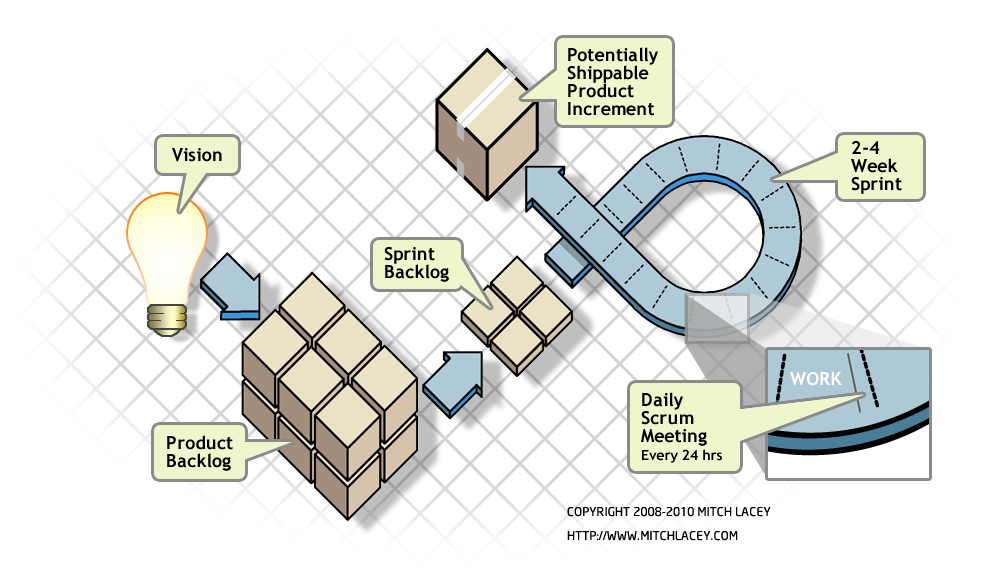
\includegraphics[width=\textwidth]{ScrumFrameworkFlow}
	\caption{Scrum Framework}
	\label{ScrumFramework}
\end{figure*}

Unsere \textbf{Vision} war die in Kapitel \ref{subsubsec:ziel} beschriebene Zielsetzung. Der Dokumentationsaufwand in der Behinderten- und Altenhilfe
soll durch die \EBP verringert werden. Das \textbf{Product Backlog} bildeten die gesamten User Stories, die bei ihrer Erstellung priorisiert wurden.
Das \textbf{Sprint Backlog} bestand in jeder Iteration aus drei bis vier User Stories. Dieses \textbf{Sprint Backlog} wurde in innerhalb einer
\textbf{Sprint} Phase abgearbeitet. Als Zeitraum für einen \textbf{Sprint} waren vier Wochen geplant, so dass nach fünf \textbf{Sprint} Phasen das
Projekt fertig entwickelt sein sollte und vier Wochen als Puffer verbleiben sollten. Zur Visualisierung des \textbf{Product} und \textbf{Sprint
Backlogs} wurden die Werkzeuge der Plattform \url{github.com} genutzt. Die Plattform bietet neben der Versionskontrolle durch das verteilte
Versionsverwaltungswerkzeugs \textit{git} auch die Möglichkeit Meilensteine mit zugehörigen Aufgaben zu definieren und diese einzelnen
Projektteilnehmern zuzuordnen. Das \textbf{Daily Scrum Meeting} wurde nicht in der vom \textit{Scrum Frameworks} vorgesehen Regelmäßigkeit und
Verbindlichkeit durchgeführt. In der ex post Betrachtung stellt sich dies als Fehler heraus. Schwierigkeiten bei der Implementierungen hätten sich
bei regelmäßiger Rücksprache untereinander sicher schneller lösen lassen. Auch eine stärkere Verbindlichkeit gegenüber den Projektzielen hätte sich
durch kontinuierliche Reflexion erzeugen lassen und zu einem besseren Produkt geführt. Eine \textbf{Shippable Product Increment} war nicht das Ziel
einer \textbf{Sprint} Phase. Allerdings sollten die User Stories des jeweiligen \textbf{Sprint Backlogs} am Ende einer \textbf{Sprint} Phase
vollständig umgesetzt sein, inklusive durchlaufener Qualitätssicherung.  


\newpage

\section{Beschreibung der Anwendung}
\label{sec:beschreibung}
\subsection{Admindialog}
\paragraph{Wohngruppe}\mbox{}\\
Im \textit{Admindialog} können Administratoren Bewohner, Wohngruppen/-heime und Mitarbeiter verwalten.
\begin{figure*}[h]
	\begin{center}
		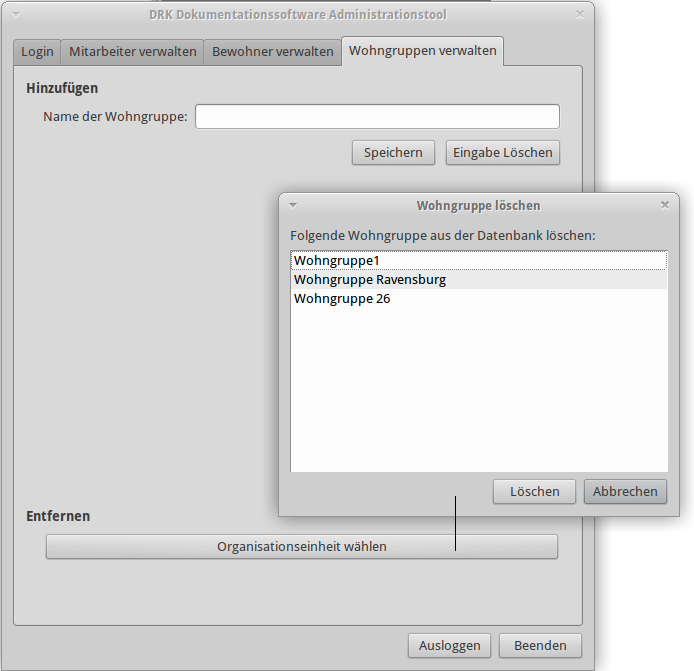
\includegraphics[keepaspectratio=true, width=0.85\textwidth]{pics/admin3.png}
		\caption{Wohngruppe}
		\label{Admindialog Wohngruppe}
		\caption{Graphen eines Interfaces}
		\label{Admindialog_Mitarbeiter_erstellen}
	\end{center}
\end{figure*}
\FloatBarrier
\noindent
Hier werden Wohngruppen erstellt, diese dienen als Gruppierung für sowohl Bewohner, als auch für Mitarbeiter.
\newpage
\noindent
\paragraph{Bewohner}\mbox{}\\
Bewohner werden mit einer Bewohnernummer, Vor-/Nachnamen und ihrer Wohngruppe  erstellt. 
\begin{figure*}[h]
	\begin{center}
		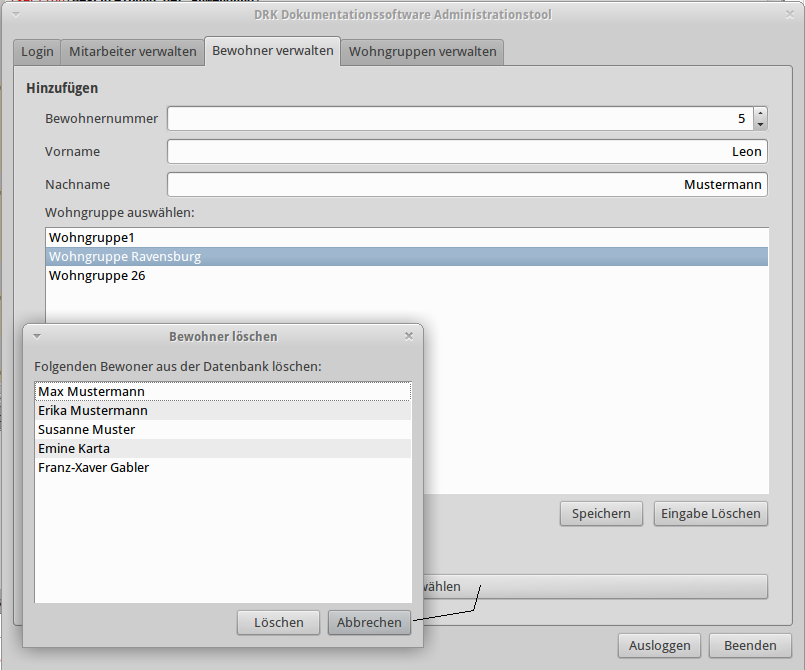
\includegraphics[keepaspectratio=true, width=0.85\textwidth]{pics/admin2.png}
		\caption{Bewohner}
		\label{Admindialog Bewohner}
		\caption{Graphen eines Interfaces}
		\label{Admindialog_Bewohner}
	\end{center}
\end{figure*}
\FloatBarrier
\noindent
Restliche Informationen werden im Client von zugewiesenen Bezugsbetreuern ausgefüllt.
\newpage
\noindent
\paragraph{Mitarbeiter}\mbox{}\\
Mitarbeiter werden mit Login sowie einigen persönlichen Daten, Name und Kontaktmöglichkeiten, sowie ihrer Berechtigung erstellt. Es ist darauf zu achten das jedem Mitarbeiter beim erstellen mindestens eine Wohngruppe zugeordnet werden muss, die er betreut. Er kann allerdings natürlich auch für mehrere Wohngruppen zuständig sein und auch der Bezugsbetreuer für Bewohner sein.
\begin{figure*}[h]
	\begin{center}
		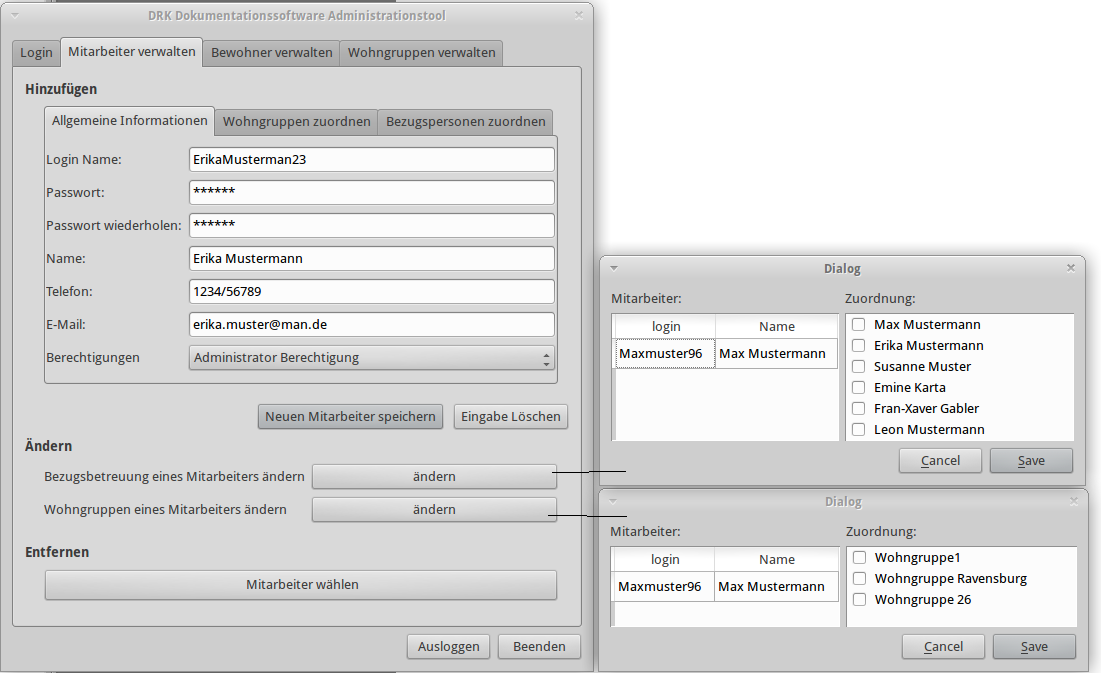
\includegraphics[keepaspectratio=true, width=0.85\textwidth]{pics/admin1.png}
		\caption{Mitarbeiter}
		\label{Admindialog Mitarbeiter}
	\end{center}
\end{figure*}
\FloatBarrier
\noindent
Mitarbeiter die keine Administratorenrechte haben können nur Informationen von Bewohner in ihrer Wohngruppe einsehen und nur von Bewohner deren Bezugsbetreuer sie sind verändern.
\newpage
\subsection{\EBP Client}
Der \EBP \textit{Client} besitzt eine widgetbasierende GUI die aus folgenden Elementen besteht.
\begin{itemize}
	\item einer Menüleiste\mbox{}\\
	\noindent
	Hier wird der Inhalt des Hauptfensters gespeichert, die zusätzlichen Widgets aus-, bzw eingeblendet oder der Mitarbeiter ausgeloggt.\\ Der Speichern Button ist ausgegraut wenn der eingeloggte Mitarbeiter kein Bezugsbetreuer des aktive Bewohners ist.
	\begin{figure*}[h]
		\begin{center}
			
\includegraphics[keepaspectratio=true, width=0.55\textwidth]{pics/client_header.png}
			\caption{Menueleiste}
			%\label{Menüleiste, fixiert an der oberen Seite des Programms}
		\end{center}
	\end{figure*}
	\FloatBarrier
	\noindent
	\item einem Informationswidget\mbox{}\\
	Hier der momentan ausgewählte Bewohner und dessen Wohngruppe angezeigt, zum ändern öffnet sich, bei Auswahl des jeweiligen Buttons, ein Popup mit allen Wohngruppen für die der Mitarbeiter berechtigt ist, bzw. alle Bewohner der jeweiligen Wohngruppe.
	\begin{figure*}[h]
		\begin{center}
			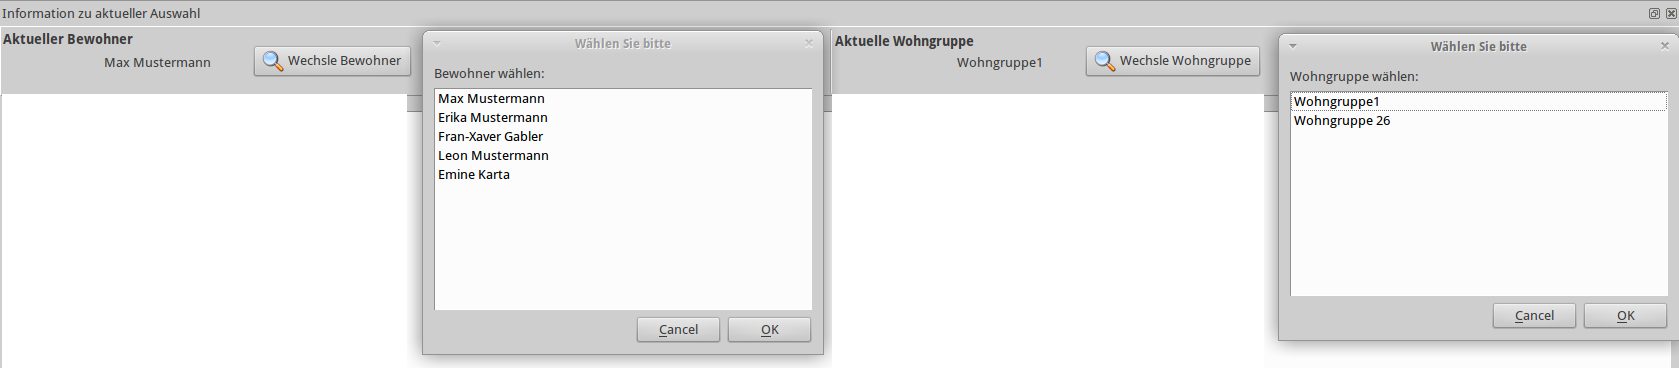
\includegraphics[keepaspectratio=true, width=0.85\textwidth]{pics/client_info.png}
			\caption{Informationswidget}
			%\label{Bewohner- und Stationswidget}
		\end{center}
	\end{figure*}
	\FloatBarrier
	\newpage
	\item einem Navigationswidget\mbox{}\\
	\noindent
	Im Navigationsmenü wird der Inhalt des Hauptfensters ausgewählt. Das ``Bewohner'' Tab enthält alle Daten und Menü's die sich auf den aktiven Bewohner beziehen, während das ``Wohngruppen'' Tab Unterpunkte beinhaltet die für die komplette aktuelle Wohngruppe gültig sind.	
	\begin{figure*}[h]
		\begin{center}
			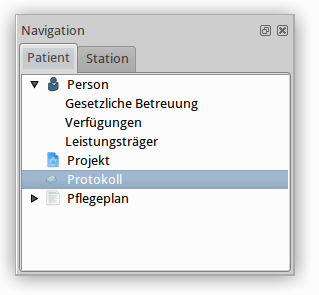
\includegraphics[keepaspectratio=true, width=0.35\textwidth]{pics/client_navi.png}
			\caption{Navigationswidget}
			%\label{Navigationsmenü}
		\end{center}
	\end{figure*}
	\FloatBarrier
	\item dem Hauptfenster\mbox{}\\
	\noindent
	Das eigentliche Hauptfenster dient zur Ein-/Ausgabe von Daten und bezieht sich immer auf den im Informationswidget ausgewählten Bewohner, bzw die ausgewählte Wohngruppe. Um hier eingegebene Daten zu sichern muss der Speichern-Knopf in der Menüleiste betätigt werden.\\
	\begin{figure*}[h]
		\begin{center}
			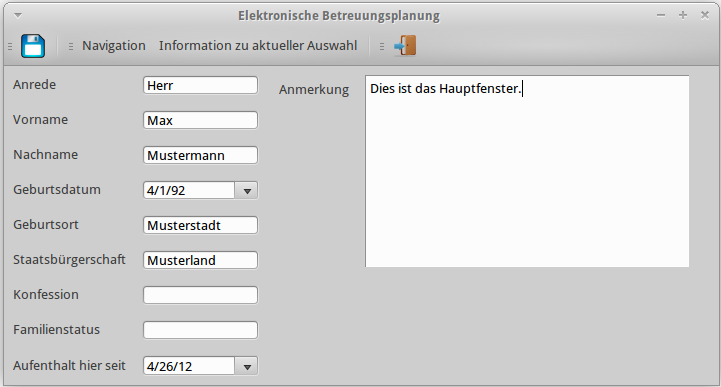
\includegraphics[keepaspectratio=true, width=0.85\textwidth]{pics/client_main.png}
			\caption{Hauptfenster}
			%\label{Hauptfenster}
		\end{center}
	\end{figure*}
	\FloatBarrier
\end{itemize}
\newpage
\subsubsection{Bewohnerbezogene Menüs}
\begin{itemize}
	\item Person\mbox{}\\
	\noindent
	Hier können persönliche Daten des Bewohners eingesehen und geändert werden.
	\begin{figure*}[h]
		\begin{center}
			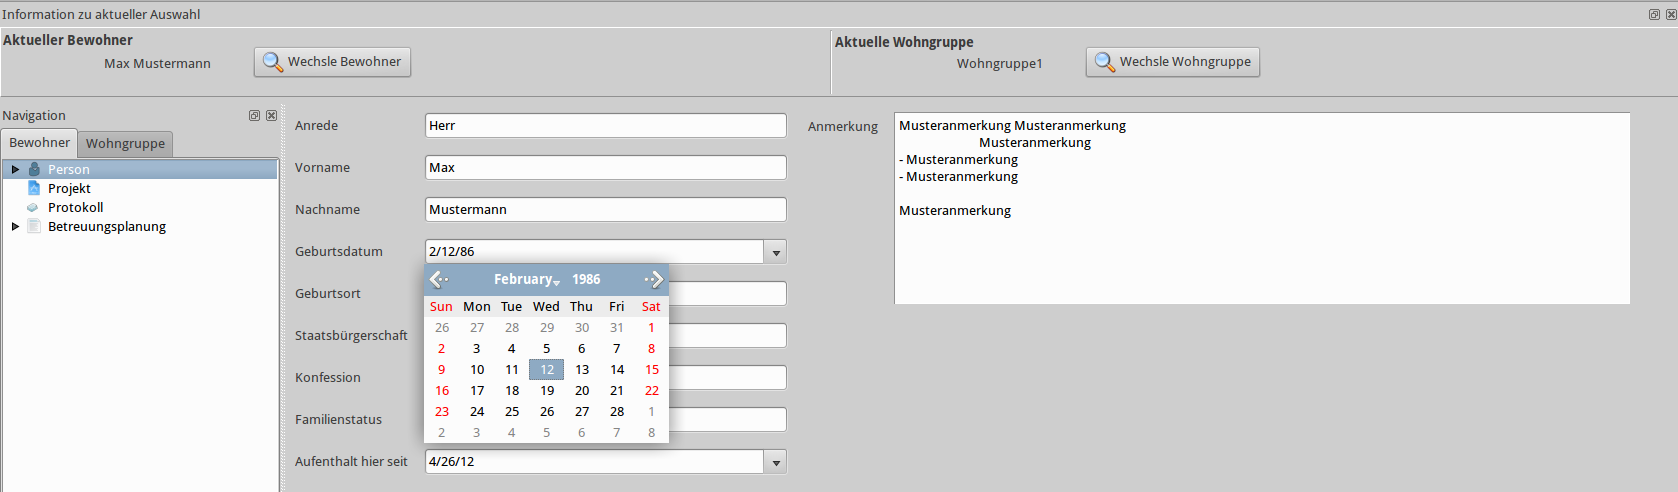
\includegraphics[keepaspectratio=true, width=0.85\textwidth]{pics/client_person.png}
			\caption{Person}
			%\label{Hauptfenster}
		\end{center}
	\end{figure*}
	\FloatBarrier
	\item Gesetzliche Betreuung\mbox{}\\
	\noindent
	Ein Unterpunkt von 'Person'. Hier sind Angaben über den gesetzlichen Betreuer des Bewohners.
	\begin{figure*}[h]
		\begin{center}
			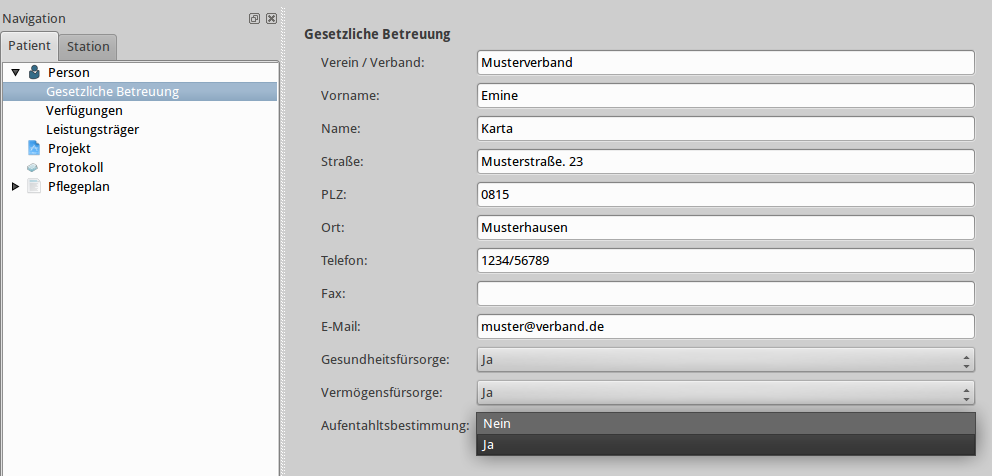
\includegraphics[keepaspectratio=true, width=0.85\textwidth]{pics/client_betreuung.png}
			\caption{Gesetzliche Betreuung}
			%\label{Hauptfenster}
		\end{center}
	\end{figure*}
	\FloatBarrier
	\newpage
	\item Verfügungen\mbox{}\\
	\noindent
	Ein Unterpunkt von 'Person'. Eventuelle Verfügungen gegen den Patienten, ihre Dauer und Begründung sind hier dokumentiert.
	\begin{figure*}[h!]
		\begin{center}
			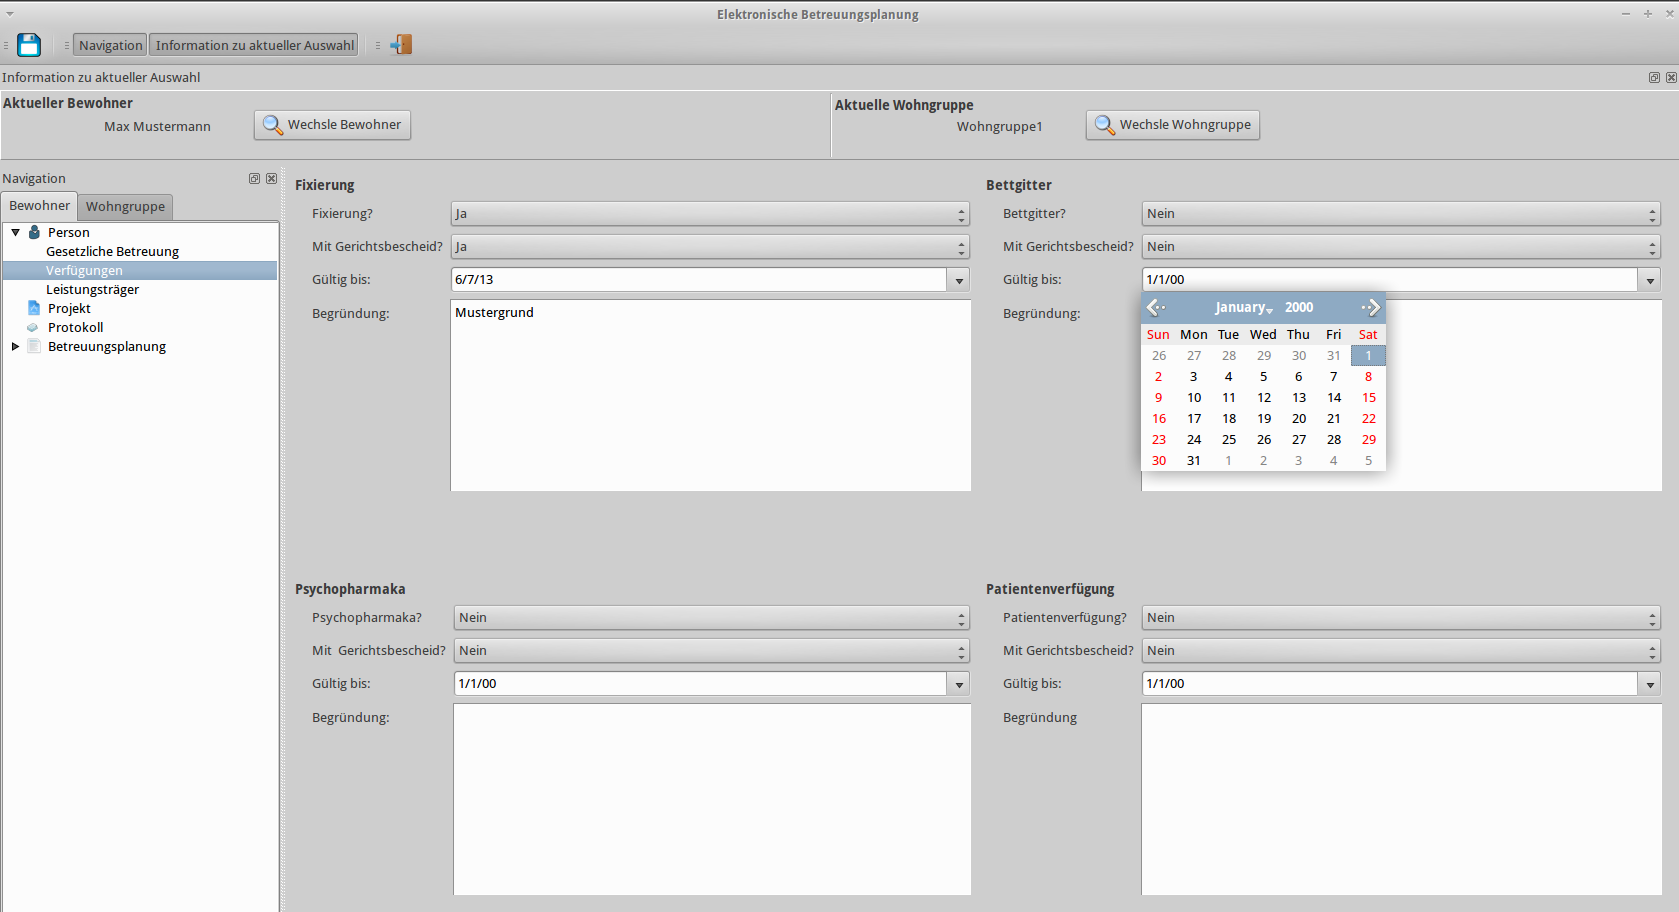
\includegraphics[keepaspectratio=true, width=0.85\textwidth]{pics/client_verfuegung.png}
			\caption{Verfügungen}
			%\label{Hauptfenster}
		\end{center}
	\end{figure*}
	\FloatBarrier
	\item Leistungsträger\mbox{}\\
	\noindent
	Ein Unterpunkt von 'Person'. Durch den Button in der links, oberen Ecke können Angabemasken für Leistungsträger hinzugefügt werden. Diese beinhalten sowohl den Leistungsträger an sich, als auch Kontaktdaten eines Ansprechspartners.
	\begin{figure*}[h!]
		\begin{center}
			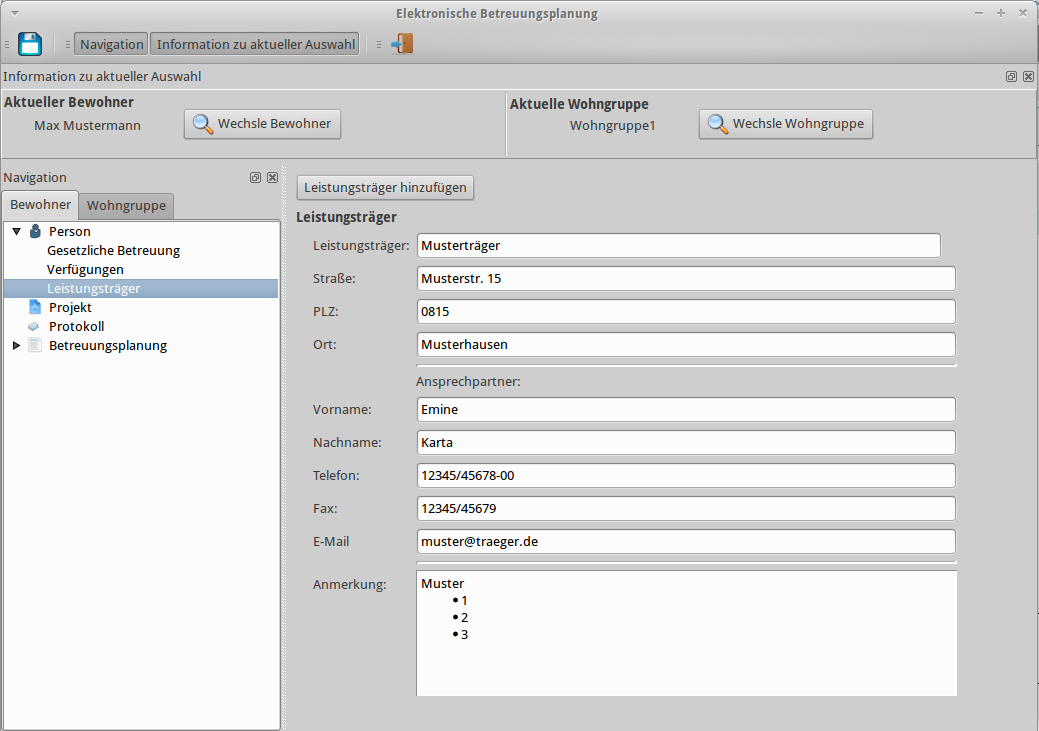
\includegraphics[keepaspectratio=true, width=0.85\textwidth]{pics/client_leistungstraeger.png}
			\caption{Leistungsträger}
			%\label{Hauptfenster}
		\end{center}
	\end{figure*}
	\FloatBarrier
	\newpage
	\item Projekt\mbox{}\\
	\noindent
	Hier werden Projekte mit Zielen, Betreuern und einer Beschreibung für den Bewohner angelegt.\\ Am unterem Rand ist eine Möglichkeit zum einfachem kopieren von ausgewählten Textteilen in die Betreungsplanung eines auswählbaren Bewohners gegeben.
	\begin{figure*}[h!]
		\begin{center}
			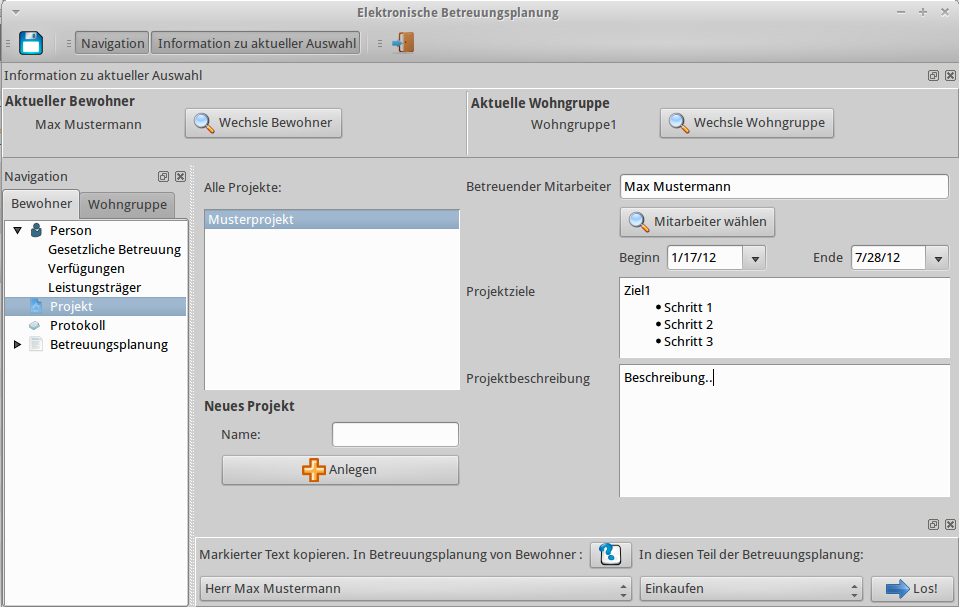
\includegraphics[keepaspectratio=true, width=0.85\textwidth]{pics/client_projekt.png}
			\caption{Projekt}
			%\label{Hauptfenster}
		\end{center}
	\end{figure*}
	\FloatBarrier
	\newpage
	\item Protokoll\mbox{}\\
	\noindent
	Um Mitarbeiterbesprechungen, die einen Bewohner betreffen, einfacher anderen betroffenen Mitarbeitern zugänglich zu machen, können hier Protokolle, durch Datum und Uhrzeit markiert, mit einer Liste der Teilnehmer sowie einer Markierung für den Schriftführer angelegt werden.\\Am unterem Rand ist eine Möglichkeit zum einfachem kopieren von ausgewählten Textteilen in die Betreungsplanung eines auswählbaren Bewohners gegeben.
	\begin{figure*}[h!]
		\begin{center}
			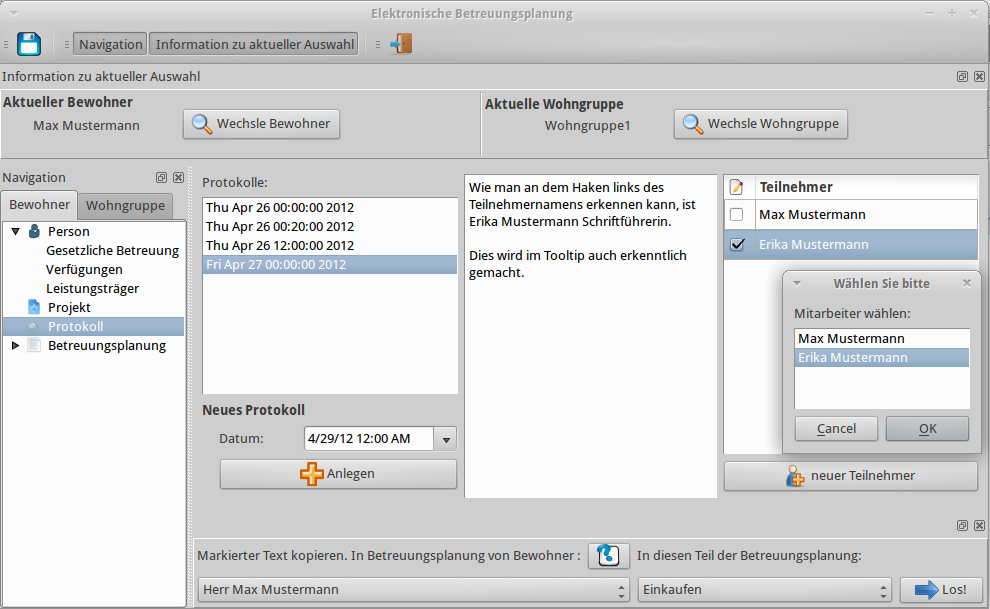
\includegraphics[keepaspectratio=true, width=0.85\textwidth]{pics/client_protokoll.png}
			\caption{Protokoll}
			%\label{Hauptfenster}
		\end{center}
	\end{figure*}
	\FloatBarrier
	\newpage
	\item Betreungsplanung\mbox{}\\
	\noindent
	in der Betreungsplanung werden einzelne Fähigkeiten oder Umstände des Bewohners beschrieben, sowohl der momentane Zustand als auch mögliche Ziele die der Bewohner erreichen soll.
	\begin{figure*}[h!]
		\begin{center}
			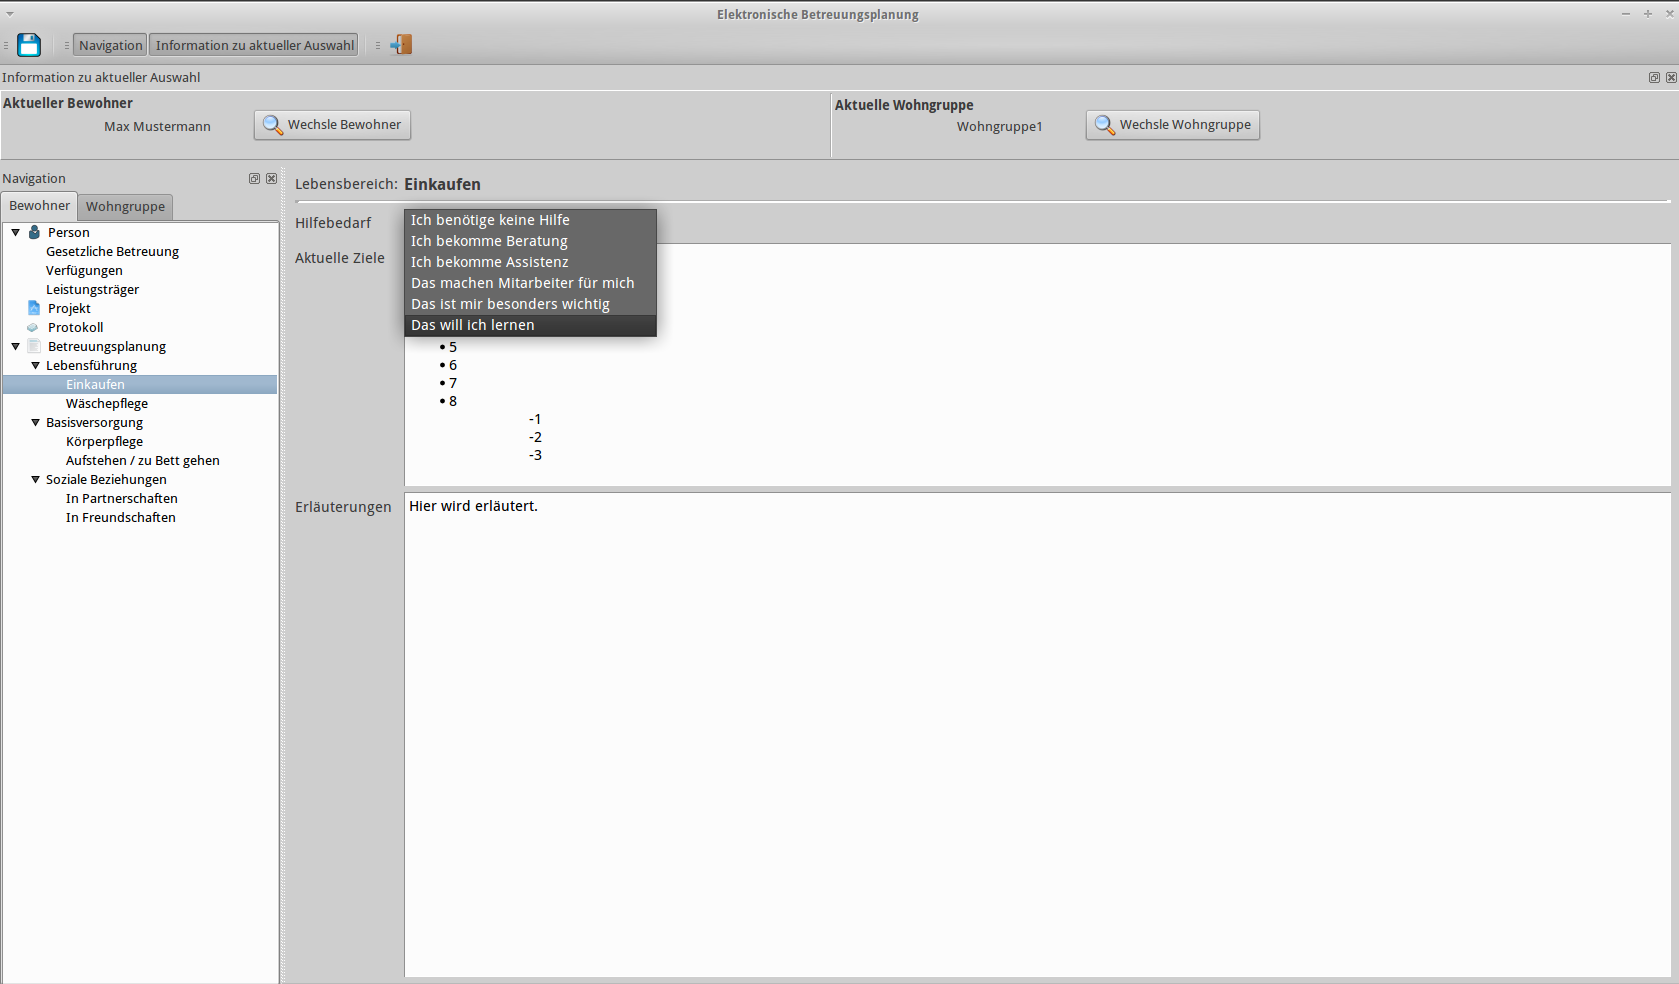
\includegraphics[keepaspectratio=true, width=0.85\textwidth]{pics/client_lebensfuehrung.png}
			\caption{Betreungsplanung: Unterpunkt Einkaufen}
			%\label{Hauptfenster}
		\end{center}
	\end{figure*}
\end{itemize}
\newpage
\subsubsection{Wohngruppen bezogene Menüs}
In den wohngruppen bezogenen Menüs können Ereignisse sowie Abwesenheiten sowohl eingetragen, als auch über Zeit filterbar eingesehen werden.
\begin{itemize}
	\item Gruppenbuch\mbox{}\\
	\noindent
	Im Gruppenbuch werden Ereignisse für andere Mitarbeiter protokolliert. Diese Ereignisse bestehen aus einem Datum, den eintragenden Mitarbeiter und einer Beschreibung.\\Standardmäßig werden alle Ereignisse, nach dem Eintragezeitpunkt sortiert, angezeigt. Es ist jedoch möglich die Einträge über einen Zeitbereich zu filtern.\\\\Am unterem Rand ist eine Möglichkeit zum einfachem kopieren von ausgewählten Textteilen in die Betreungsplanung eines auswählbaren Bewohners gegeben.
	\begin{figure*}[h]
		\begin{center}
			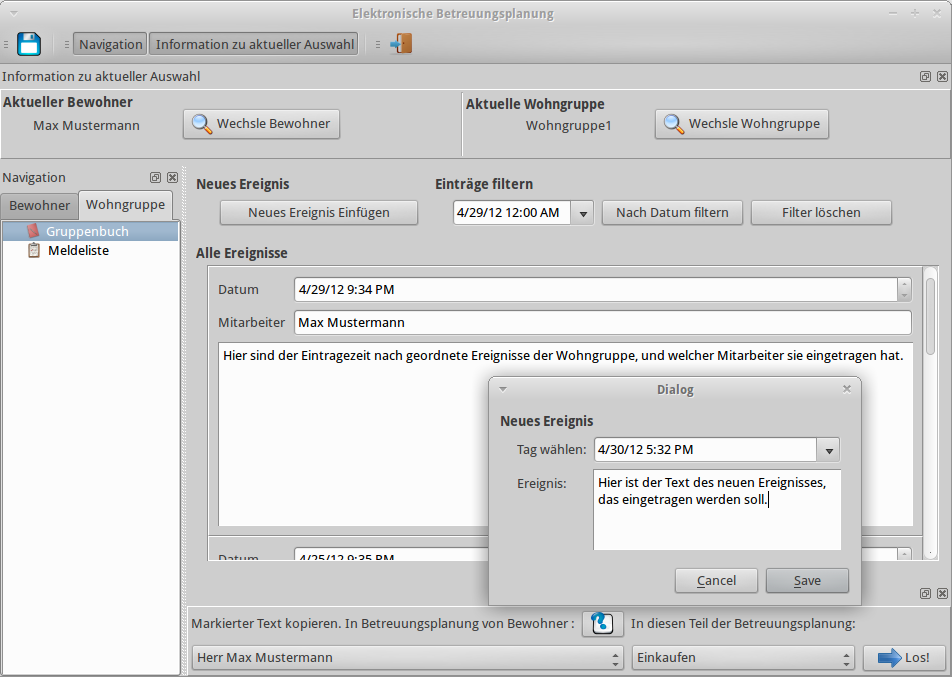
\includegraphics[keepaspectratio=true, width=0.85\textwidth]{pics/client_ereignis.png}
			\caption{Gruppenbuch}
			%\label{Hauptfenster}
		\end{center}
	\end{figure*}
	\FloatBarrier
	\newpage
	\item Meldeliste\mbox{}\\
	\noindent
	In der Meldeliste werden alle Bewohner der Wohngruppe die zu dem ausgewählten Tag bereits in der Wohngruppe waren angezeigt. Standardmäßig sind alle Bewohner als 'Anwesend' eingetragen. Es ist nur möglich Bewohner als abwesend zu markieren, wenn ein Grund angegeben wird.\\ Es ist möglich die Abwesenheiten der Bewohner in einem auswählbaren Zeitbereich zu exportieren. Dieser Export ist sowohl im CSV-Format (zur weiterverarbeitung in anderen Programmen, z.B. Excel) als auch in From einer Textdatei die in einer druckbaren Formatierung möglich.
	\begin{figure*}[h]
		\begin{center}
			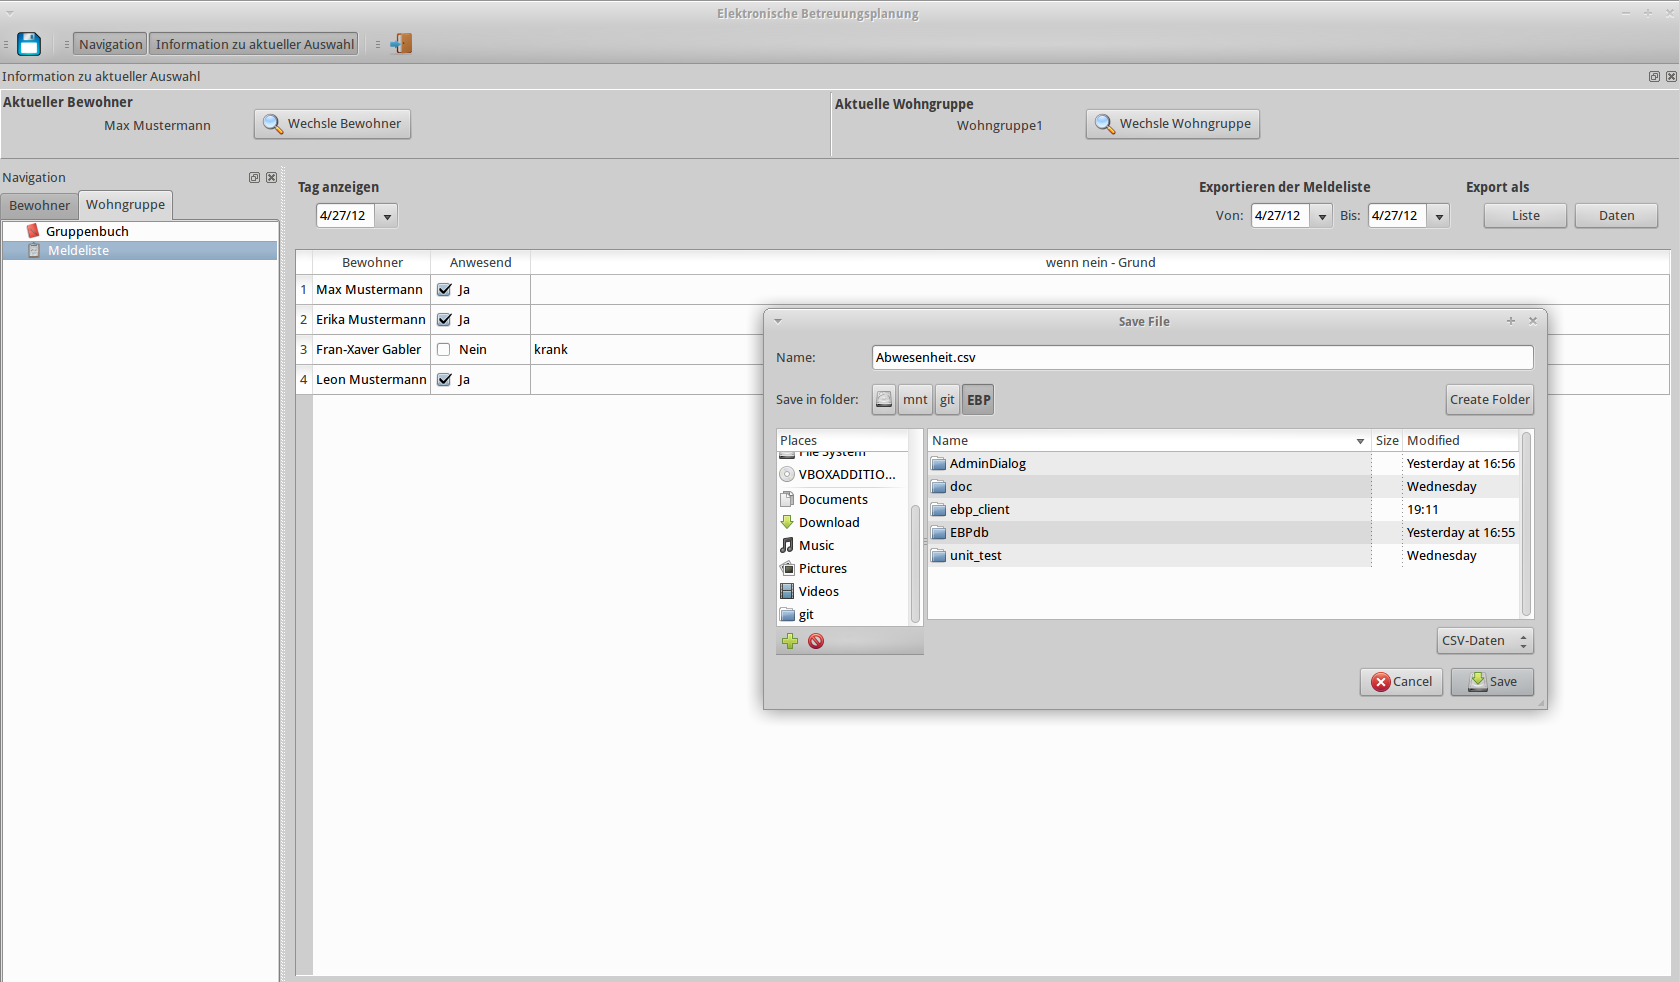
\includegraphics[keepaspectratio=true, width=0.85\textwidth]{pics/client_meldeliste.png}
			\caption{Meldeliste}
			%\label{Hauptfenster}
		\end{center}
	\end{figure*}
	\FloatBarrier
\end{itemize}
\newpage
\subsection{Lokalisierung}
Sowohl der AdminDialog als auch die \EBP sind koplett lokalisierbar. Qt stellt dafür einen einfachen Mechanismus zur Verfügung. Jeder zu
lokalisierende String wird dabei von einem Makro umschlossen. Mit Hilfe des Qt Linguist können diese Strings zu einem Wörterbuch zusammengefasst und
übersetzt werden. Für die \EBP war im Plichtenheft angedacht, ein englisches und eine deutsches Wörterbuch zur Verfügung zu stellen. In den
Gesprächen zur Anforderungsdefinition mit Herrn Zimmer zeichnete sich ein anderer Lokalisierungsbedarf an die \EBP ab.\\
Die Fachkräfte in der Altenhilfe und der Behindertenhilfe haben ihre eigene Fachsprache im täglichen Umgang mit ihren Klienten. So liegt der Fokus in
der Altenhilfe eher auf pflegerischen Tätigkeiten, wohingegen in der Behindertenhilfe pädagogische Ziele und Maßnahmen im Fordergrund stehen. Ein
Klient wird in der Altenhilfe eher als Patient bezeichnet, in der Behindertenhilfe spricht man häufiger von einem Bewohner. Um diesen Umstand zu
berücksichtigen, wurden keine Wörterbücher für Englisch und Deutsch erstellt, sondern Wörterbücher für die Altenhilfe und für die Behindertenhilfe.\\
Wird der Client oder der AdminDialog ohne Parameter gestartet, wird das Wörterbuch der Behindertenhilfe geladen. Um die Lokalisierung der Altenhilfe
zu aktivieren, muss der entsprechenden Anwendung der Parameter ``-a'' übergeben werden.

\newpage

\subsection{Erstellen der Anwendung}
\subsubsection{Abhängigkeiten}
\paragraph{Zur Laufzeit:}
\begin{itemize}
	\item \textbf{odb} - ODB Laufzeitbibliothek
	\item \textbf{odb-mysql} - MySQL Backend für ODB
	\item \textbf{odb-qt} - QT integration für ODB
	\item \textbf{qt} - QT Framework
\end{itemize}
\paragraph{Zur Compilezeit:}
\begin{itemize}
	\item \textbf{CMake} - Buildsystem
	\item \textbf{ODB Toolchain} - Enthält den Precompiler
	\item \textbf{GCC} - GNU Compiler Collection
\end{itemize}
\subsubsection{Kompilieren der Quellen}
Die komplette Anwendung kann im Wurzelverzeichnis des Projekts gebaut werden:\\
\begin{lstlisting}
$ cmake .
\end{lstlisting}
Generiert das benötigte Makefile.\\
Ist dies erfolgreich abgeschlossen, wird mit\\
\begin{lstlisting}
$ make
\end{lstlisting}
der eignetliche Kompiliervorgang gestartet.\\
\subsubsection{Vorbereiten der Datenbank}
Um die Datenbank zu initialisieren befindet sich ein Shell-Script im EBPdb Verzeichnis:\\
\begin{lstlisting}
$ ./initDB.sh -u root -p "DATENBAKNAME"
\end{lstlisting}


\newpage

\section{Technische Realisierung}

\subsection{Architektur}
Das Projekt ist in folgende Module aufgeteilt:
\begin{itemize}
	\item EBP-Client - Grafisches Datenbankfrontend für den alltäglichen Gebrauch
	\item AdminDialog - Grafisches Datenbank-Administrationswerkzeug
	\item libEBPdb - Stellt Fachklassen und Persistenzfunktionen als Bibliothek zur Verfügung
	\item Unit-Tests - Automatisierte Tests der Bibliothek
\end{itemize}

\newpage

\subsection{Qt als Grafikbibliothek}

\newpage

\subsection{Buildsystem}
Da das Projekt \textit{Qt} als einen zentralen Bestandteil verwendet, ist es naheliegend das \textit{Qt}-eigene Buildsystem \textit{QMake} einzusetzen. Insbesondere die Verwendung von \textit{QMake} innerhalb des \textit{QtCreator}s kann die Entwicklung einfacher Anwendungen erleichtern.\\
Eine bedeutende Schwierigkeit von \textit{QMake} ist es jedoch, komplexere Build-Prozesse zu automatisieren, wie beispielsweise die Integration des verwendeten \textit{ORM}s in den Build-Vorgang der Persistenzschicht.\\
Daher wurde in diesem Projekt ein zweigleisiges Buildsystem eingesetzt:\\
Zum einen lassen sich die GUI-Anwendungen weiterhin mit \textit{QMake} erstellen. Zum anderen kann das komplette Projekt samt Bibliothek der Persistenzschicht mit \textit{CMake} kompiliert werden.\\

\newpage

\subsection{Persistenzschicht mit ODB (libEBPdb)}

\subsubsection{Object-Relational-Mapping (ORM)}
Um die Daten einer relationellen Datenbank auf Objekte innerhalb einer Programmiersprache abzubilden gibt es prinzipiell zwei Ansätze.
Entweder wird der Code der die Eigenschaften eines Objekts aus der Datenbank liest und schreibt manuell implementiert, oder aber es wird ein Mechanismus eingesetzt, der automatisiert Variablen eines Objekts den Feldern einer Datenbank zuordnet (Object-Relational-Mapping).\\
Das Einsetzen eines solchen Mappers hat den Vorteil, dass der sich oft wiederholende Code zum Laden und Speichern der Daten von und in die Datenbank reduziert werden kann. Dies führt zu wartbarerem Code, der bei Änderungen an der Datenbankstruktur schneller und fehlerfreier anpassbar ist.

\subsubsection{Auswahl des Verwendeten Mappers}
Das verwendete Qt4-Toolkit enthält zwar eine plattformunabhängige Schnittstelle für Datenbanken (QtSql), jedoch hat diese keine ORM Funktion.
Folgende ORM-Systeme wurden in Betracht gezogen\\
\url{http://en.wikipedia.org/wiki/List_of_object-relational_mapping_software}:
\begin{itemize}
	\item LiteSQL - Datenbankschema wird mit XML Dateien beschrieben
	\item ODB - Datenbankschema wird aus den C++ Klassen generiert
	\item QxOrm - Benutzt QtSql; Unter Umständen müssen direkte Aufrufe von QtSql erfolgen. \cite{QxOrm_Tutorial}
\end{itemize}
Alle Systeme bieten eine Qt Integration, die die Schnittstelle zwischen GUI und Persistenzschicht vereinfachen.
Ebenso unterstützen alle Systeme mehrere Datenbankbackends.
Letztendlich fiel die Entscheidung auf ODB, da diese Bibliothek (unter anderem durch Caching) die beste Performance verspricht.
Außerdem lassen sich Klassen mit geringem Aufwand persistent machen.

\newpage

\subsubsection{Code-Generierung}
Kern des verwendeten Object-Relational-Mappers ODB ist ein spezieller Precompiler, der auf bestimmte Precompiler-Pragmas reagiert.
Durch das Markieren einer Klassendefinition mit einer Pragma-Direktive können persistente Objekte der Klasse erstellt werden:\\
\begin{lstlisting}
#pragma db object
class Mitarbeiter { ... }
\end{lstlisting}
Der ODB-Compiler generiert daraufhin Code, der das gegebene Objekt auf eine Datenbankstruktur abbilden kann. Des weiteren wird auch die Datenbankstruktur in Form von SQL-Dateien generiert, die direkt an die verwendete Datenbank weitergereicht werden können um alle zur Laufzeit benötigten Tabellen zu erstellen. Auf diese Weise wird ebenso sichergestellt, dass Datenbank und Anwendung stets die selbe Struktur verwenden.\\
\begin{figure*}[htp!]
	\begin{center}
		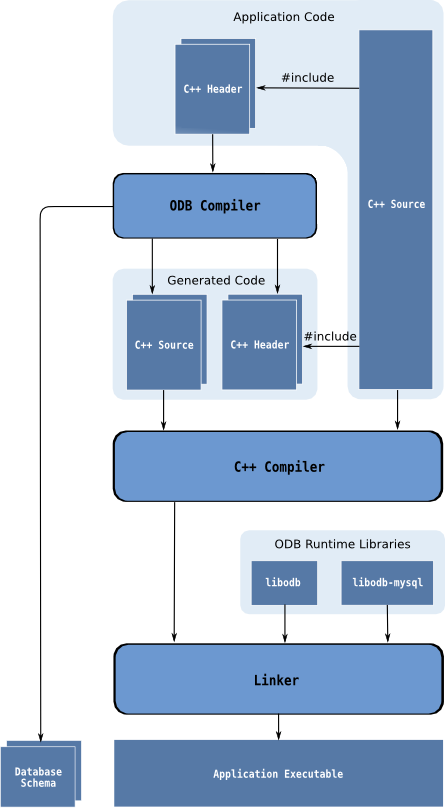
\includegraphics[width=0.4\textwidth]{odb-flow}
	\end{center}
	\caption{ODB Toolchain \cite{ODB_Manual}}
	\label{ODB-Flow}
\end{figure*}

\newpage

\subsubsection{Datenbankunabhängigkeit}
Durch die zusätzliche Abstraktionsschicht ist es einfacher die bestehende Persistenzschicht auf ein neues Datenbanksystem zu portieren.\\
Die umgesetzte Lösung ist weitestgehend frei von datenbankspezifischen Aufrufen, und benutzt ausschließlich die Schnittstelle des eingesetzten Object-Relational-Mappers.
Lediglich das User-Management, um ``Mitarbeiter`` auf Datenbankbenutzer abzubilden verwendet Datenbankspezifische SQL-Kommandos, die über ODB abgewickelt werden.

\subsubsection{Integration in das Buildsystem}
Um das Buildsystem (CMake) automatisch bei Veränderungen des Quellcodes alle für ODB benötigten Dateien generieren zu lassen, wird im Buildscript wie folgt vorgegangen:
\begin{enumerate}
\item Suchen aller Dateien die ODB spezifische Pragma-Definitionen beinhalten.
\item Erstellen einer Vorschrift um für jede so gefundene Datei den ODB-Compiler aufzurufen.
	Dabei werden auch die Abhängigkeiten der generierten Dateien korrekt in das Buildsystem eingefügt, so dass diese nur neu generiert werden, wenn tatsächlich Änderungen an der jeweiligen Eingangsdatei oder deren Abhängigkeiten vorhanden sind.
\end{enumerate}
Der entsprechende Auszug aus dem CMake Buildscript:\\
\lstset{language=clean}
Jeder zum Projekt gehörende C++ Header wird eingelesen und nach ODB-Pragma-Definitionen durchsucht:
\begin{lstlisting}
foreach( header ${EBPdb_headers} )
	file( READ ${header} headercontent )
	if( "${headercontent}" MATCHES "#pragma[ \t]+db[ \t]+object" )
\end{lstlisting}
Für jede gefundene Datei wird die generierte ODB-Datei zu den zu kompilierenden Quelldateien hinzugefügt:
\begin{lstlisting}
		get_filename_component( headerbase ${header} NAME_WE )
		set( EBPdb_sources ${EBPdb_sources} ${headerbase}-odb.cxx )
\end{lstlisting}
Damit der ODB-Precompiler den Quellcode korrekt parsen kann, müssen sämtliche verwendeten Include-Verzeichnisse bei dem Aufruf des Precompilers angegeben werden. Die Projekteinstellungen werden hierfür übernommen:
\begin{lstlisting}
		get_directory_property( odbincludes INCLUDE_DIRECTORIES )
		foreach( includedir ${odbincludes} )
			set( odbincludeargs ${odbincludeargs} -I${includedir} )
		endforeach( includedir )
\end{lstlisting}
Eine Regel zum Ausführen des Precompilers der der die Quellcode-Datei generiert wird erstellt (gleichzeitig werden auch alle weiteren benötigten Dateien erzeugt):
\begin{lstlisting}
		add_custom_command( OUTPUT ${headerbase}-odb.cxx ${headerbase}-odb.hxx ${headerbase}-odb.ixx ${headerbase}.sql
			COMMAND odb ${odbincludeargs} --database mysql --profile qt --generate-query --generate-schema ${header}
			DEPENDS ${header} )
	endif( "${headercontent}" MATCHES "#pragma[ \t]+db[ \t]+object" )
endforeach( header )
\end{lstlisting}


\newpage

\subsubsection{Datenbankschema}
\begin{figure*}[htp!]
	\begin{center}
		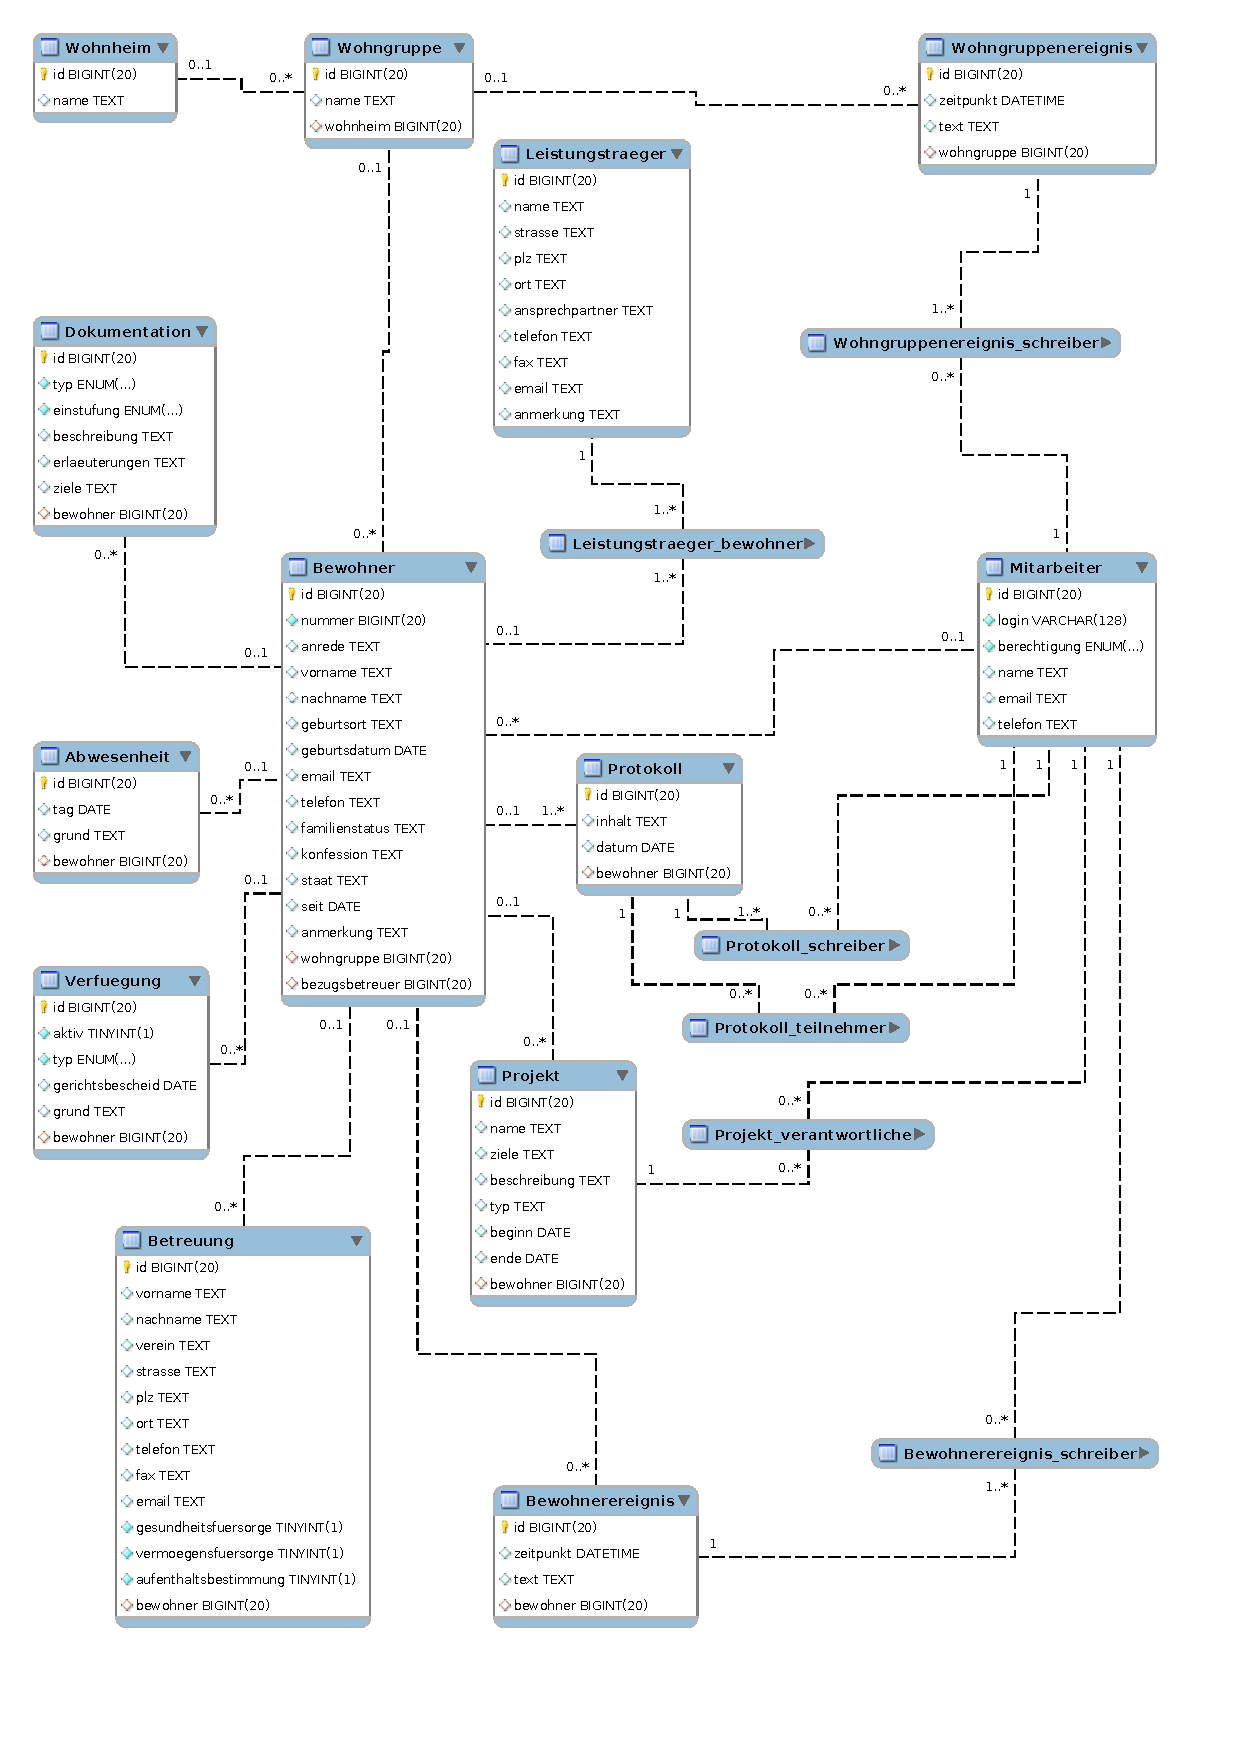
\includegraphics[width=0.93\textwidth]{scheme}
	\end{center}
	\caption{Datenbankschema als ER Diagramm}
	\label{ERDiagram}
\end{figure*}

\subsubsection{Abstraktion der Schnittstelle}
\lstset{language=c++}
Zweck der Bibliothek ist es die internen Abläufe des ORM Systems zu verbergen, und der Anwendung eine einfache, objektorientierte Schnittstelle zur Verfügung zu stellen.\\
Voraussetzung zur Verwendung der Bibliothek ist eine funktionierende Verbindung zur Datenbank:\\
\begin{lstlisting}
QSharedPointer<ebp::connection> connection =
	QSharedPointer<ebp::connection>
	(
		new ebp::connection( "LoginName", "DatenbankName", "localhost", 3306)
	);
connection->establish( "PasswortDesBenutzers" );
QSharedPointer<Mitarbeiter> mitarbeiter = connection->mitarbeiter();
\end{lstlisting}
Sollen neue Mitarbeiter auf die Datenbank zugreifen, kann mit\\
\begin{lstlisting}
QSharedPointer<ebp::Mitarbeiter> neuerMitarbeiter =
	QSharedPointer<ebp::Mitarbeiter>
	(
		new ebp::Mitarbeiter( "LoginName", ebp::Mitarbeiter::WohngruppenRecht, "Name" )
	);
neuerMitarbeiter->create( connection, "PasswortDesNeuenMitarbeiters" );
\end{lstlisting}
ein neuer Mitarbeiter in der Datenbank erstellen. Gleichzeitig wird auch ein neuer Datenbankbenutzer angelegt, der intern mit den Daten des Mitarbeiters verknüpft wird.
Der Datenbankbenutzer erhält dabei nur die Berechtigungen an den Datenbanktabellen, die er für seinen ''Rechtestatus`` benötigt.\\
\\
Analog zum Erstellen eines Mitarbeiters, lassen sich auch alle anderen Objekte der Bibliothek erzeugen:\\
\begin{lstlisting}
QSharedPointer<ebp::Bewohner> bewohner =
	QSharedPointer<ebp::Bewohner>
	(
		new ebp::Bewohner( 0 )
	);
bewohner->create( connection );
\end{lstlisting}
Veränderungen eines Objekts lassen sich mit der ''update``-Methode in der Datenbank sichern:\\
\begin{lstlisting}
bewohner->telefon( "0123456789" );
bewohner->update( connection );
\end{lstlisting}
Verknüpfungen lassen sich mit den jeweiligen ''link``-Methoden herstellen:\\
\begin{lstlisting}
ebp::Bewohner::linkBezugsbetreuer( bewohner,mitarbeiter);
ebp::Bewohner::linkWohngruppe( bewohner, wohngruppe);
bewohner->update( connection );
\end{lstlisting}
Dabei geht eine Verknüpfung immer von einer der Klassen aus - die andere ist das ''inverse`` Gegenstück.
Um die Verknüpfung persistent zu machen, muss immer die ''update``-Methode der Klasse verwendet werden, von der die Verknüpfung ausgeht.\\
Angelegte verknüpfungen lassen sich mit den verschiedenen ''load``-Methoden wieder laden:\\
\begin{lstlisting}
QList< QSharedPointer<ebp::Projekt> > projekte = bewohner->loadProjekte( connection );
\end{lstlisting}

\newpage

\subsection{Unit-Tests}

Unit-Tests, auch Komponententests genannt, sind sehr entwicklungsnahe Tests und sollen sicherstellen, dass die Erwartungen an eine Software erfüllt
werden können, indem Fehler vermieden werden.\\
''Das Testen von Software dient durch die Identifizierung von Defekten und deren anschließender Beseitigung zur Steigerung der Softwarequalität. Die 
Testfälle sollen so gewählt werden, dass sie weitgehend der späteren Benutzung der Software entsprechen. Die nachgewiesene Qualität des
Programmswährend der Tests entspricht dann der zu erwartenden Qualität während der späteren Benutzung\cite[S. 11]{Softwaretests}.''\\

Bei Unit-Tests werden einzelne Programmmodule isoliert von einander getestet. Dadurch sollen Einflüsse durch andere Softwarekomponenten ausgeschlossen
werden. Programmmodule müssen dabei aber nicht zwingendermaßen nur einzelne Klassen oder Funktionen sein \cite[Vgl. S. 11]{Softwaretests}. Bei der
\EBP erfolgt die Trennung in die Programmmodule libEBPdb und GUI. Für die Qualitätssicherung der GUI-Funktion wurden keine automatisierter Testcode
eingesetzt. Die korrekte Funktionalität der GUI wurde durch das regelmäßige Testen aller Masken durch einen Tester gewährleistet. Sollen auch diese
Aufgaben automatisiert werden, stellt Qt eine beschränkte API für User Interface Tests zur Verfügung. Darüber hinaus gibt es auch weitere
Drittanbieter für Tools und Frameworks zum automatisierten Testen von User Interfaces, wie z.B. TestComplete von Smart Bear. Diese Tests sind
allerdings äußerst aufwendig zu konfigurieren und zu pflegen.\\

Es wurden daher in erster Linie die libEBPdb mit Hilfe von automatisierten Unit-Tests getestet. Es sollte eine Testumgebung entworfen werden, die es
dem Entwickler ermöglicht nach einer Änderung im Quellcode mit Hilfe eines einzelnen Befehls überprüfen zu können, ob die libEBPdb als Gesamtheit noch
korrekt ausgeführt wird. Dazu wurde die Testumgebung mit Hilfe des Testtools CTest, ein Teil von CMake, in das Buildsystem integriert. Als Framework
für die eigentlichen Unit-Tests kommt die QTestLib, ein Teil von Qt, zum Einsatz. QTestLib bietet diverse Makros, die ein errechnetes Ergebnis mit dem
erwarteten Wert vergleichen und ein abweichendes Verhalten protokollieren. Dies ist die grundlegende Vorgehensweise bei einem Unit-Test. So
vergleicht der folgende Aufruf des Macros QCOMPARE den Rückgabewert einer Methode der Klasse ebp::Wohngruppe mit dem erwarteten Wert. Im Fehlerfall
wird der Rückgabewert und die Fehlerstelle protokolliert.
\begin{lslisting}
QCOMPARE(wohngruppenEreignisList.at(i)->zeitpunkt(),QDateTime(QDate(2012,4,1),QTime(11,11)));
\end{lslisting}



\newpage

\subsection{Eingesetzte Entwurfsmuster}
\subsubsection{Mediator Pattern - Der Text Transfer Agent}
Neben der Verwaltung von klienten- und wohngruppenspezifischen Daten ist die Überführung von Textstücken aus verschiedenen Teilen des
Dokumentationsprogramms die Hauptfunktion der \EBP. Diese Funktion wird im folgenden \textit{Text Transfer} genannt. \newline
Der \textit{Text Transfer} soll aus den Masken Bewohner$\rightarrow$Protokoll, Bewohner$\rightarrow$Projekt und Wohngruppe$\rightarrow$Gruppenbuch
erfolgen. Gespeichert werden die Textfragmente in den verschiedenen Feldern der Betreuungsplanung eines beliebigen Bewohners. Die Unterschiedlichkeit
der Quellen für die zu transferierende Textfragmente und die Variation an Zielfelder war die Schwierigkeit bei der Implementierung dieser
Funktionalität. Da die Anzahl an Objekten, die als Quelle dienen, im Programmverlauf stark variieren kann, muss der Lösungsansatz sehr flexibel
implementiert sein. Abbildung \ref{unstrukturiert} zeigt die Vielzahl an möglichen Kommunikationswegen zwischen den einzelnen Objekten.\\
\begin{figure*}[htp!]
	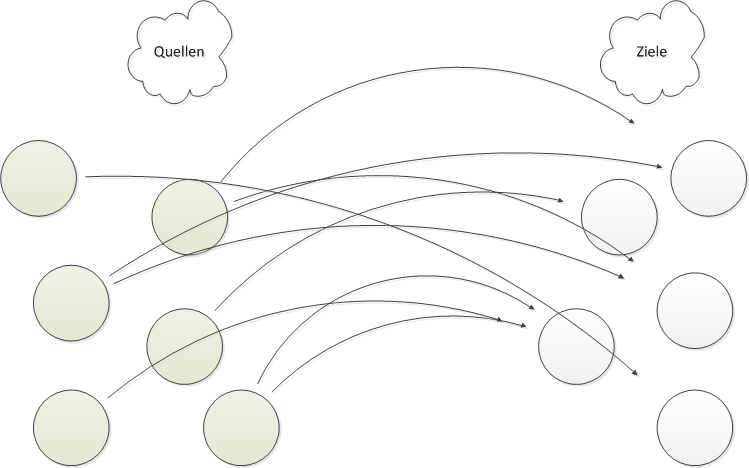
\includegraphics[width=0.8\textwidth]{unmediated}
	\caption{Kommunikationswege zwischen Objekten}
	\label{unstrukturiert}
\end{figure*}
Um nicht jeden Kommunikationsweg einzeln verwalten zu müssen, wurde der \textit{Text Transfer} in Form des Mediator Patterns entworfen. Den Zweck
eines Mediators definiert GAMMA wie folgt: \\
``Define an object that encapsulates how a set of objects interact. Mediator promotes loose coupling by keeping objects from reffering to each other explicitly, 
and it lets you vary their interaction independently \cite[S. 273]{Entwurfsmuster}.''\\
\\
\textbf{Beteiligte Objekte\cite[S. 277]{Entwurfsmuster}:}
\begin{enumerate}
	\item Eine Instanz des TextTransferAgent als konkreter Mediator. Auf eine abstrakte Mediatorklasse wurde auf Grund des klar definierten Aufgabengebiets verzichtet.
	\begin{enumerate}
		\item Implementiert die Interaktion zwischen den verschiedenen Kollegen.
		\item Kennt alle zu verwaltenden Kollegenobjekte.
		\item Deklaration der Mediatorklasse TextTransferAgent:
		\begin{lstlisting}
class TextTransferAgent : public QFrame
{
    Q_OBJECT

public:
    explicit TextTransferAgent(QList<TextTransferInterface *>Interfaces,const SessionContext &context, QWidget *parent = 0);
    ~TextTransferAgent();
    void registerNewInterface(TextTransferInterface *newInterface);

private slots:
    void on_bewohnerBox_currentIndexChanged(int index);
    void on_losButton_clicked();
    void on_helpButton_clicked();

private:
    const SessionContext &_context;
    Ui::TextTransferAgent *ui;
    QSharedPointer< ebp::Bewohner > selectedBewohner;
    QList < QSharedPointer < ebp::Dokumentation > > dokus;
    QList<TextTransferInterface *> textInterfaces;
};
		\end{lstlisting}
	\end{enumerate}
	\item Beliebig viele Instanzen von Klassen, die das TextTransferInterface implementiert haben als Kollegen.
	\begin{enumerate}
		\item Jeder Kollege kennt das Mediatorobjekt.
		\item Möchte ein Kollege mit einem anderen kommunizieren, tut er dies über den Mediator.
		\item Die Kommunikation zwischen den Kollegen ist in dieser Implementierung unidirektional. Klassen, die das TextTransferInterface implementiert haben dienen stets 
			als Quelle für den Texttransfer. Als Ziel für den Texttransfer stehen dem Meditor über das aktive Bewohner Objekt alle Instanzen der Betreuungsplanung zur Verfügung.
		\item Deklaration des Kollegeninterfaces TextTransferInterface:
		\begin{lstlisting}
class TextTransferInterface
{
public:
    virtual TextTransferInformation getSelectedText()=0;
};
		\end{lstlisting}
	\end{enumerate}
\end{enumerate}
Abbildung \ref{strukturiert} zeigt die Kommunikationswege eines Texttransfers zwischen den einzelnen Objekten, koordiniert durch ein Mediatorobjekt. 
\begin{figure*}[htp!]
	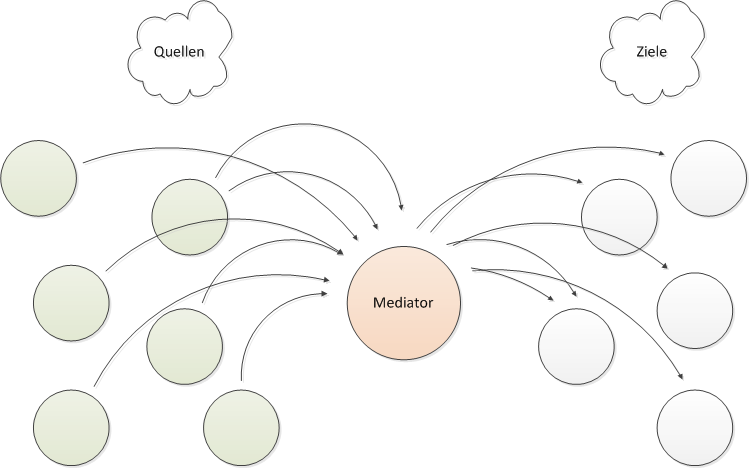
\includegraphics[width=0.8\textwidth]{mediated}
	\caption{Kommunikationswege zwischen Objekten, koordiniert durch einen Mediator}
	\label{strukturiert}
\end{figure*}
\subsubsection{Observer Pattern - Signal Slot Konzept}
Ein klassisches Konzept zur Kommunikation zwischen Objekten stellen \textit{Events} und \textit{Eventhandler} dar. Dieses Konzept ist allerdings nicht typsicher und unflexibel, da es für ein \textit{Events} auch nur einen \textit{Eventhandler} geben kann\cite[S. 32]{Qt4}. Qt hingegen nutzt zur Kommunikation zwischen Objekten das \textit{Signal Slot Konzept}, das wie ein Observer Pattern aufgebaut ist. GAMMA beschreibt das Observer Pattern wie folgt: \\
"Define a one-to-many dependency between objects so that when one object changes state, all its dependents are notified and updated automatically\cite[S. 293]{Entwurfsmuster}."\\
Qt realisiert dies, indem Funktionen einer Klasse durch das Schlüsselwort \textit{Slot} gekennzeichnet werden können. Diese \textit{Slots} werden mit einem \textit{Signal} verbunden und sind damit als \textit{Observer} zu betrachten. Das \textit{Subject} ist ein Funktionsprototyp, der durch das Schlüsselwort \textit{Signal} gekennzeichnet wird. Dieser Prototyp wird nicht implementiert. GAMMA beschreibt diese Beziehung folgendermaßen:\\
''The Subject is the publisher of notifications. It sends out these notifications without having  to know who its observers are. Any number of observers can subscibe to receive notifications\cite[S. 294]{Entwurfsmuster}."\\
Verbunden wird ein \textit{Signal} mit einem \textit{Slot} durch den Aufruf der statischen Methode QObject::connect(). \textit{Signal} und \textit{Slot} müssen dabei die gleichen Argumente besitzen. Dadurch wird die Typsicherheit gewährleistet. Allerdings sind die Schlüsselworte \textit{Signal} und \textit{Slot} kein reines C++. Klassen die sich diesem Konzept bedienen müssen daher durch den \textit{Meta Object Compiler (MOC)} in Standard-konformes C++ verwandelt werden\cite[Vgl. S. 51]{Qt4}.
\EBP bedient sich dieses Konzepts an vielen Stellen. Der Anmeldevorgang soll hier als Beispiel dienen. Die Anmeldung an dem Client erfolgt auf einer Maske, die durch die Klasse LoginForm beschrieben wird. Diese Klasse definiert auch ein eigenes \textit{Signal} \textit{validLogin()}:
\begin{lstlisting}
class LoginForm : public QWidget
{
    ...
signals:
    void validLogin(QSharedPointer<ebp::Mitarbeiter> newMitarbeiter, QSharedPointer<ebp::connection> newConnection);
    ...
};
\end{lstlisting}
Die Klasse MainWindow definiert den dazu passenden \textit{Slot}, der nach einer erfolgreichen Anmeldung den Client initialisiert:
\begin{lstlisting}
class MainWindow : public QMainWindow
{
    ...
private slots:
    void validLogin(QSharedPointer<ebp::Mitarbeiter> newMitarbeiter, QSharedPointer<ebp::connection> newConnection);
    ...
};
\end{lstlisting}
Durch dieses Konzept der losen Kopplung könnten bei Bedarf weitere \textit{Slots} an ein erfolgreiches Anmelden angekoppelt werden, ohne auf den bereits bestehenden \textit{Slot} zum initialisieren des Clients Einfluss zu nehmen.
\subsubsection{Model/View Pattern - Datenvisualisierung}
Das Entwurfsmuster Model/View oder auch Model/View/Controller ist ein klassisches Entwurfsmuster der Softwareentwicklung und beschreibt, wie die Datenhaltung, die Visualisierung der Daten und die Interaktion mit dem Benutzer in verschiedenen Komponenten realisiert wird. Ziel dieses Entwurfsmusters ist es, flexiblen und wiederverwendbaren Programmcode zu entwickeln.
Das Framework Qt bietet die Variante des Model/View Entwurfsmusters an. Dabei werden Der Controller und der View in der selben Komponente realisiert. Dies vereinfacht die Handhabung, ermöglicht aber immernoch ein Trennen der Datenhaltung und der Visualisierung der Daten \cite[Vgl.]{QtModelView}.
Qt bietet Abstrakte Klassen für ein Table-, List- oder Treemodel an, um grundlegene Funtionalitäten für die entsprechenden Views vorzugeben. Sind diese Ansätze nicht flexibel genug, kann QAbstractItemModel implementiert werden. Um die Mitarbeiterobjekte in einem Tableview darstellen zu können, wurde ein einfaches Model mit Hilfe von QAbstractTableModel implementiert:
\begin{lstlisting}
class EmployeeTableModel : public QAbstractTableModel
{
    Q_OBJECT
    QList < QSharedPointer < ebp::Mitarbeiter > > EmployeeList;
public:
    explicit EmployeeTableModel(QList < QSharedPointer < ebp::Mitarbeiter> > employees, QObject *parent = 0);
    
    // Überschriebene Funktion. Liefert dem View die Anzahl an Zeilen    
    int rowCount(const QModelIndex &parent) const;

    // Überschriebene Funktion. Liefert dem View die Anzahl an Spalten
    int columnCount(const QModelIndex &parent) const;

    // Überschriebene Funktion. Liefert dem View die Daten.
    QVariant data(const QModelIndex &index, int role) const;

    // Überschriebene Funktion. Liefert dem View die Überschriften.
    QVariant headerData(int section, Qt::Orientation orientation, int role);
    QSharedPointer < ebp::Mitarbeiter> getMitarbeiter(int index);
    void addMitarbeiter(QSharedPointer<ebp::Mitarbeiter> newMitarbeiter);
};
\end{lstlisting}
Dieses Model kann in verschiedenen Tableviews verwendet werden. Die Views können sich stark von einander unterscheiden. Über die überschriebenen Funktionen von QAbstractTableModel wird sichergestellt, dass der View auf die richtigen Daten zugreift.
\newpage


\newpage

\bibliography{refs}
\bibliographystyle{plainnat}

\end{document}
